\section{Experimental Results}

This section evaluates the performance and limitations of our approach
for the three case studies described in Section~\ref{sec:methodology},
and provides a comparison to state-of-the-art approaches. First we
show that \textsc{ProGraML}, unlike prior state-of-the-art approaches
to machine learning over code, is capable of replicating core compiler
analysis tasks that are key to optimization. Second, we improve upon
prior approaches to the task of heterogeneous device mapping. Finally,
we set a new state of the art in the difficult task of classifying
program algorithms, and ablate the contribution of the structure and
content of the \textsc{ProGraML} representation.


\subsection{Case Study A: Compiler Analysis}

Table~\ref{table:data_flow_results} summarizes the performance of the
\textsc{ProGraML} approach when tasked with learning a suite of
benchmark compiler analysis, along with the performance of a
state-of-the-art sequential approach, DeepTune$_\text{IR}$. As a
binary classification task, compiler analyses display an extreme class
imbalance as only a small fraction of a program graph is typically
relevant to computing the result set of an analysis. On our datasets,
an accuracy of 96.6\% can be achieved by always predicting the
negative class. For this reason we report only binary precision,
recall, and $F_1$ scores with respect to the positive class.

\begin{table}
  \centering%
  \footnotesize
\renewcommand{\arraystretch}{1.6}
\begin{tabular}{L{2.45cm} L{3.1cm} L{3.2cm} L{1.6cm} | R{1.3cm} R{1cm} R{1cm}}
  \toprule
  \textbf{Problem} & \textbf{Analysis type} & \textbf{Example optimization} & \textbf{Model} & \textbf{Precision} & \textbf{Recall} & $\bm{F_1}$\\
  \hline
  \multirow{2}{2.45cm}{\textsc{Reachability}} &
    \multirow{2}{3.1cm}{Forwards, control flow only} &
    \multirow{2}{3.2cm}{Dead code elimination}
        & DeepTune$_{\text{IR}}$ & 0.520 & 0.497 & 0.504\\
                  & & & ProGraML & \textbf{0.997} & \textbf{0.995} & \textbf{0.996}\\
  \hline
  \multirow{2}{2.45cm}{\textsc{DomTree}} &
    \multirow{2}{3.1cm}{Backwards, control flow only} &
    \multirow{2}{3.2cm}{Global Code Motion}
        & DeepTune$_{\text{IR}}$ & 0.721 & 0.081 & 0.138\\
                  & & & ProGraML & \textbf{0.985} & \textbf{0.693} & \textbf{0.781}\\
  \hline
  \multirow{2}{2.45cm}{\textsc{DataDep}} &
    \multirow{2}{3.1cm}{Backwards, control and data flow} &
    \multirow{2}{3.2cm}{Instruction scheduling}
        & DeepTune$_{\text{IR}}$ & 0.999 & 0.136 & 0.236\\
                  & & & ProGraML & \textbf{1.000} & \textbf{0.988} & \textbf{0.993}\\
  \hline
  \multirow{2}{2.45cm}{\textsc{Liveness}} &
    \multirow{2}{3.1cm}{Backwards, control and data flow} &
    \multirow{2}{3.2cm}{Register allocation}
        & DeepTune$_{\text{IR}}$ & --- & --- & ---\\
                  & & & ProGraML & \textbf{1.000} & \textbf{0.999} & \textbf{0.999}\\
  \hline
  \multirow{2}{2.45cm}{\textsc{Subexpressions}} &
  \multirow{2}{3.1cm}{Forwards, statement and operand values and positions} &
  \multirow{2}{3.2cm}{Global Common Subexpression Elimination}
      & DeepTune$_{\text{IR}}$ & \textbf{1.000} & 0.123 & 0.214 \\
                & & & ProGraML & 0.965 & \textbf{0.925} & \textbf{0.930} \\
  \hline
  \multirow{2}{2.45cm}{\textbf{Average}} &
  \multirow{2}{3.1cm}{---} &
  \multirow{2}{3.2cm}{---}
      & DeepTune$_{\text{IR}}$ & 0.810 & 0.209 & 0.273\\
                & & & ProGraML & \textbf{0.989} & \textbf{0.920} & \textbf{0.940}\\
  \hline
\end{tabular}
%
  \vspace{.7em}
  \caption{%
    Benchmark compiler analyses results using two approaches: (a)
    DeepTune$_{\text{IR}}$, a sequential model adapted to work at the
    LLVM-IR level for statement-level classification, and (b)
    \textsc{ProGraML}, our approach. The relational representation
    significantly outperforms a sequential approach across all
    problems. For the Global Common Subexpressions analysis,
    DeepTune$_{\text{IR}}$ achieved a higher precision than
    \textsc{ProGraML} by predicting only the root statement as a
    component in a subexpression, avoiding false-positives.\\*
  }%
  \label{table:data_flow_results} %
\end{table}

As can be seen in Table~\ref{table:data_flow_results}, the relational
representation of our approach, coupled with learning through
iterative message passing, yields models that far outperform the
state-of-the-art sequential approaches to modeling code.  The grouping
of program tokens by statement performed by DeepTune$_\text{IR}$
offers a more restrictive classification interface than with
\textsc{ProGraML} (where data elements are also represented as graph
vertices). As such, it is not able to perform the per-variable
classification required for \textsc{Liveness}
analysis\footnote{Theoretically the same approach for grouping
  embeddings by statement could also be extended to group all
  statements by variables, but this would require duplicating many
  statements in the input representation, increasing the length of the
  sequences far beyond what we can practically process using a
  sequential model.}. For fairness, we exclude \textsc{Liveness} from
LSTM aggregate values in Table~\ref{table:data_flow_results}. Despite
this, \textsc{ProGraML} achieves an average 94.0 $F_1$, versus 27.3
$F_1$ for DeepTune$_\text{IR}$.

In many cases, the sequential model regresses to a classification mode
in which only the source vertex is labeled as positive, yielding poor
recall.  The \textsc{ProGraML} models achieve both high precision and
high recall in all tasks except \textsc{DomTree}, where recall is
comparatively poor. When model performance is considered as a function
of the number of training graphs, as shown in
Figure~\ref{fig:dataflow_convergence}, we see that the performance of
the \textsc{ProGraML} models quickly convergences towards near-perfect
$F_1$ score on a holdout validation set, except in the case of
\textsc{DomTree}, where the model is still improving at the end of
training. This suggests estimating the \emph{transfer} and \emph{meet}
operators of this backwards analysis poses a greater challenge for the
network, which may require further training.

\begin{figure}
  \begin{subfigure}{\linewidth}
    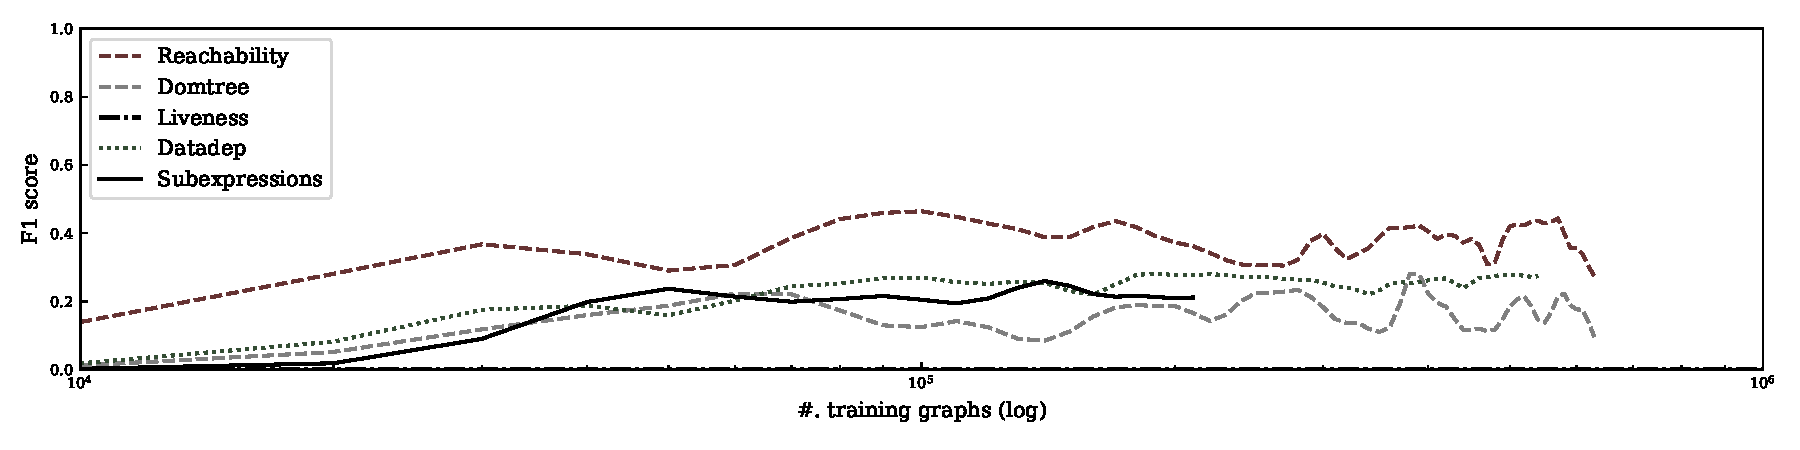
\includegraphics[width=\linewidth]{images/dataflow-lstm.pdf}
    \caption{DeepTune$_{\text{IR}}$}
    \label{fig:dataflow-lstm-f1}
  \end{subfigure}
  \\*
  \begin{subfigure}{\linewidth}
    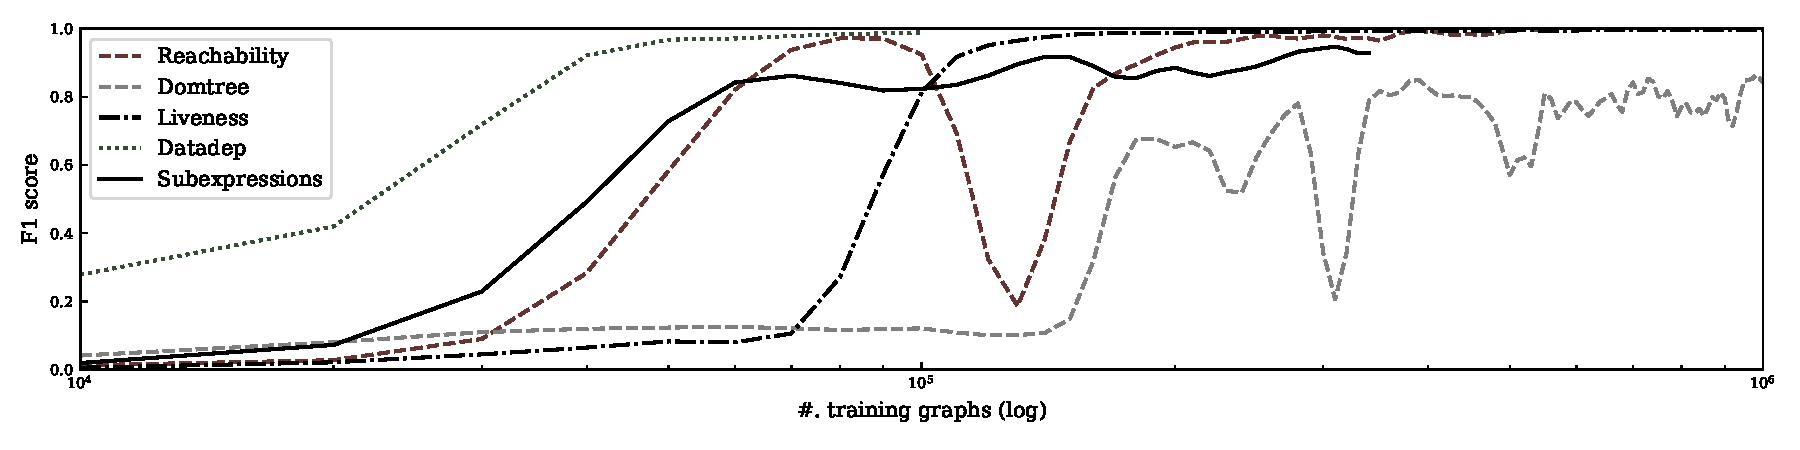
\includegraphics[width=\linewidth]{images/dataflow-ggnn.pdf}
    \caption{\textsc{ProGraML}}
    \label{fig:dataflow-ggnn-f1}
  \end{subfigure}
  \caption{%
    The $F_1$ score of compiler analysis models on a 20k-graph
    validation set as a function of the number of training graphs from
    10k to 1M. Each model was given six hours to train on a machine
    with a GTX 1080 GPU, with early termination if accuracy on the
    validation set reached 99.99\%. We have applied a Gaussian filter
    ($\sigma=1$) to aid in visualizing the trends in each set of
    scores.  }
  \label{fig:dataflow_convergence}
\end{figure}

Table~\ref{tab:confusion_matrices} shows confusion matrices for the
per-vertex classification of \textsc{ProGraML} models on the test
set. While the distribution of errors is balanced for
\textsc{Reachability}, in the case of \textsc{Domtree} and
\textsc{Subexpressions} the ratio of false negatives ($T_+P_-$)
outweighs the false positives ($T_-P_+$), indicating that models favor
under-approximating the value sets of these analyses. This may be an
artifact of training with such a large imbalance towards negatives
($T_-$) over positive ($T_+$) class labels. In future work we will
explore addressing this class imbalance by selecting multiple root
points on a graph for analysis simultaneously, thereby increasing the
size of the value set to include multiple (possibly overlapping)
regions.

\begin{table}
  \centering
\scriptsize
\renewcommand{\arraystretch}{1.5}
\begin{subfigure}{.19\linewidth}
  \centering
  \begin{tabular}{r | c c}
    \toprule
    & $\bm{P_-}$ & $\bm{P_+}$ \\
    \midrule
    $\bm{T_-}$ & 96.64\% & 0.01\% \\
    $\bm{T_+}$ & 0.01\% & 3.34\% \\
    \bottomrule
  \end{tabular}
  \caption{\textsc{Reachability}}
\end{subfigure}
\hfill
\begin{subfigure}{.19\linewidth}
  \centering
  \begin{tabular}{r | c c}
    \toprule
    & $\bm{P_-}$ & $\bm{P_+}$ \\
    \midrule
    $\bm{T_-}$ & 95.94\% & 0.13\% \\
    $\bm{T_+}$ & 1.70\% & 2.23\% \\
    \bottomrule
  \end{tabular}
  \caption{\textsc{DomTree}}
\end{subfigure}
\hfill
\begin{subfigure}{.19\linewidth}
  \centering
  \begin{tabular}{r | c c}
    \toprule
    & $\bm{P_-}$ & $\bm{P_+}$ \\
    \midrule
    $\bm{T_-}$ & 98.80\% & 0.00\% \\
    $\bm{T_+}$ & 0.00\% & 1.20 \% \\
    \bottomrule
  \end{tabular}
  \caption{\textsc{DataDep}}
\end{subfigure}
\hfill
\begin{subfigure}{.19\linewidth}
  \centering
  \begin{tabular}{r | c c}
    \toprule
    & $\bm{P_-}$ & $\bm{P_+}$ \\
    \midrule
    $\bm{T_-}$ & 90.00\% & 0.00\% \\
    $\bm{T_+}$ & 0.00\% & 9.99\% \\
    \bottomrule
  \end{tabular}
  \caption{\textsc{Liveness}}
\end{subfigure}
\hfill
\begin{subfigure}{.19\linewidth}
  \centering
  \begin{tabular}{r | c c}
    \toprule
    & $\bm{P_-}$ & $\bm{P_+}$ \\
    \midrule
    $\bm{T_-}$ & 99.12\% & 0.02\% \\
    $\bm{T_+}$ & 0.13\% & 0.73\% \\
    \bottomrule
  \end{tabular}
  \caption{\textsc{Subexpressions}}
\end{subfigure}
  \caption{%
    Confusion matrices for compiler analyses using
    \textsc{ProGraML}. Rows denote true negative ($T_-$) and true
    positive ($T_+$), columns denote predicted negative ($P_-$) and
    predicted positive ($P_+$). The value of a cell is the ratio of
    per-vertex model outputs of this type, e.g. $T_-P_+$ is the ratio
    of false positives.%
  }
  \label{tab:confusion_matrices}
\end{table}


\subsection{Case Study B: Heterogeneous Device Mapping}

The performance of ProGraML and baseline models is shown in
Table~\ref{figure:devmap_results}. We reused the pre-trained
inst2vec-embeddings for the NCC baseline that were published with the
original work, however all models themselves have been reimplemented
to ensure fair comparison across different models under a unified
evaluation regime and absolute performance numbers can thus deviate
from the original publications.

Baseline models were trained with hyperparameters from the original
works. For the \textsc{ProGraML} results we used 6 layers in the GGNN
corresponding to 6 timesteps of message propagation, while sharing
parameters between even and odd layers to introduce additional
regularization of the weights. We ran a sweep of basic hyperparameters
which led us to use the pre-trained inst2vec statement
embeddings~\cite{Ben-nun2018} and to exclude the use of position
representations. Both of these hyperparameter choices help
generalization by reducing the complexity of the model. This is not
surprising in light of the fact that the dataset only contains 680
samples derived from 256 unique programs. \textsc{ProGraML} was
trained with the Adam optimizer with default parameters, a learning
rate of $10^{-3}$ and a batch size of 18,000 nodes for 300 epochs
(resulting in ca. 12000 iteration steps of the
optimizer). Additionally we found dropout~\cite{Srivastava2014} with a
rate of $0.1$ on the weights of the message propagation function to be
beneficial on the validation set as well. For the \textsc{ProGraML}
result, we repeat the automated sweep for all hyperparameter
configurations and picked the configuration with the best average
validation performance. Performance on the unseen tenth of the data is
reported.

As can be seen, \textsc{ProGraML} outperforms prior approaches to this
problem by all metrics (accuracy, precision, recall, and $F_1$),
across both device datasets.


\begin{table}
  \centering%
  \centering
\footnotesize
\renewcommand{\arraystretch}{1.6}
\begin{subfigure}{.48\linewidth}
\begin{tabular}{l llll}
  \toprule
  % See sheets programl_devmap/tags
   & Accuracy & Precision & Recall & $F_1$\\
  \midrule
  Static Mapping                 & 58.8\% & 0.35 & 0.59 & 0.44\\
  DeepTune~\cite{Cummins2017b}   & 71.9\% & 0.72 & 0.72 & 0.72\\
  DeepTune$_{\text{IR}}$         & 73.8\% & 0.76 & 0.74 & 0.75\\
  NCC~\cite{Ben-nun2018}    & 80.3\% & 0.81 & 0.80 & 0.80\\
  ProGraML                       & \textbf{86.6}\% & \textbf{0.89} & \textbf{0.87} & \textbf{0.88}\\
  \midrule
\end{tabular}
\caption{AMD}
\end{subfigure}
\begin{subfigure}{.48\linewidth}
\begin{tabular}{l llll}
  \toprule
   & Accuracy & Precision & Recall & $F_1$\\
  \midrule
  Static Mapping                 & 56.9\%    & 0.32 & 0.57 & 0.41\\
  DeepTune~\cite{Cummins2017b}   & 61.0\%    & 0.69 & 0.61 & 0.65\\
  DeepTune$_{\text{IR}}$         & 68.4\% & 0.70 & 0.68 & 0.69\\
  NCC~\cite{Ben-nun2018}    & 78.5\%   & 0.79 & 0.79 & 0.79\\
  ProGraML                       & \textbf{80.0}\% & \textbf{0.81} & \textbf{0.80} & \textbf{0.80}\\
  \midrule
\end{tabular}
\caption{NVIDIA}
\end{subfigure}
  \caption{%
    Five approaches to predicting heterogeneous device mapping: (a)
    Static Mapping (b) DeepTune~\cite{Cummins2017b}, a sequential
    model using tokenized OpenCL, (c) DeepTune$_{\text{IR}}$, the same
    model adapted for tokenized LLVM-IR, (d) NCC, which uses
    pre-trained statement embeddings, and (e) \textsc{ProGraML}, our
    approach.%
  }%
  \label{figure:devmap_results} %
\end{table}


\subsection{Case Study C: Algorithm Classification}

Table \ref{tab:classify} summarizes the algorithm classification
accuracy results of our method and baselines.

\paragraph{Baseline Experiments} Lifting the XFG graph representation
from pretraining embeddings~\cite{Ben-nun2018} to the high-level task
of algorithm classification showed a strong improvement of
performance. We found that jointly learning the embeddings with the
model from scratch (cf. \emph{XFG-rnd} in Table \ref{tab:classify})
outperformed both fixed inst2vec embeddings (\emph{XFG-i2v}) as well
as finetuning of inst2vec embeddings (not shown). Both baselines are
an improvement over inst2vec and show that graph-based models are more
suited to the task than models with less structure.

Next, we want to understand whether our particular
graph-representation reached its design goals and can provide
additional improvement on POJ104.

\paragraph{\textsc{ProGraML} Experiments} To ablate the contribution
of the tokenization from the performance boost provided by the
\textsc{ProGraML} representation itself, we include a GGNN-based
\emph{structure-only baseline} (denoted as \emph{GGNN-s}) of our
approach, where the only information on each node is whether it
represents a statement or an identifier in the graph, but we refrain
from tokenizing statements.  We think that algorithm classification is
a problem that lends itself especially well to judging the power of
the representation \emph{structure}, since most algorithms are
well-defined independent of implementation details, such as datatypes.

The results in Table \ref{tab:classify} show that the structure alone
of our \textsc{ProGraML} representation is sufficient to outperform
the XFG baselines and prior work on the task of algorithms
classification. Adding inst2vec statement tokenization further
improves performance. This suggests that there is room for improvement
in performance by extending the graph encoding method to achieve
better vocabulary coverage and stronger generalization. We leave this
to future work.

\begin{table}
  \centering
  \footnotesize
  %\vspace{0.2cm}
  \begin{tabular}{lllllllll}
    \toprule
        & TBCNN~\cite{Mou2016} & NCC~\cite{Ben-nun2018} & \multicolumn{2}{c}{XFG} & \multicolumn{3}{c}{ProGraML}\\
    \cmidrule(lr){4-5} \cmidrule(lr){6-8}
    Metric & & & i2v & rnd  & GGNN-s & GGNN & Transformer\\
    \midrule
    Test Error [\%] & 6.0 & 5.17 & 4.56 & 4.29 & 3.87 & 3.78 & \textbf{3.33}\\
    Improvement [\%] & --- & 0.0 & 11.8 & 17.0 & 25.1 & 26.9 & \textbf{35.6}\\
    \bottomrule
    \vspace{.7em}
  \end{tabular}
  \caption{%
    Algorithm Classification Error on POJ-104 \cite{Mou2016}. The two
    XFG models are distinct only in their embedding layers:
    \emph{XFG-i2v} uses inst2vec embeddings, while \emph{XFG-rnd}
    jointly learns the embeddings. The results denoted by Surface
    Features and TBCNN are reproduced from Mou et al. \cite{Mou2016}.%
  }
  \label{tab:classify}
\end{table}
